Aurinkosähköjärjestelmät koostuvat aurinkopaneeleista, aurinkoinverttereistä sekä mahdollisista energiavarastoista. Riippuen järjestelmästä, aurinkopaneeliketjuun tai yksittäisiin paneeleihin voidaan kytkeä myös DC/DC-muunnin. Tästä saadaan lisähyötyjä varjostustilanteissa tai epätasaisessa auringonpaisteessa.  Kuvassa 2.1 näkyy aurinkosähköjärjestelmän lohkokaavio, joka esittää verkkokytketyn järjestelmän komponentteja.
\begin{figure}
  \centering
  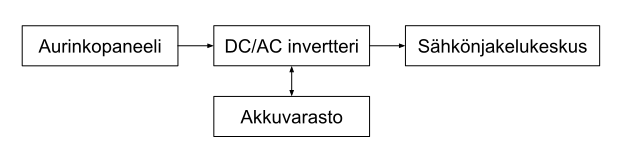
\includegraphics[width=0.75\textwidth]{figures/PV_system_components_1}
  \caption{Aurinkosähköjärjestelmän komponentit}
\end{figure}

Järjestelmä tuottaa energiaa vain tiettyyn aikaan päivästä, ja sen tuottoteho voi vaihdella hyvin nopeasti säätilasta riippuen. Kotitaloudessa nimellisteholtaan päiväsajan minimikulutusta suuremmat järjestelmät, joissa ei ole hyödynnetty kommunikaatiorajapintoja, syöttävät huipputehoaikana sähköä verkkoon päin. Kommunikaatiorajapintoja hyödyntämällä kotitaloudet voisivat hyödyntää tämän energian itse, liittämällä aurinkosähköjärjestelmän esimerkiksi kodin automaatioon. Tällöin kodista saataisiin myös energiaomavaraisempi, kun ostosähkön määrä olisi pienempi.

Järjestelmän koko, mahdolliset staattiset varjostuskohdat sekä tulevaisuuden laajentamistarpeet vaikuttavat järjestelmän suunnitteluun. Invertterin valinta vaikuttaa laite- ja asennuskustannuksiin sekä järjestelmän päivittäiseen energiantuotantoon, mutta myös järjestelmän turvallisuuteen ja suojalaitteiden tarpeeseen. Inverttereiden eri vaihtoehtoja käsitellään myöhemmin omassa kappaleessaan.

Lähes kaikki verkon käyttöpaikat ovat verkonhaltijan sähkömittarin takana. Mikäli alle 100kVA:n tehoinen tuotantolaitos sijaitsee sähkönkäyttöpaikalla, jossa on kaksisuuntainen tuntimittauslaite, ei tuotantolaitokselle tarvitse asentaa erillistä mittaria. Muussa tapauksessa tuotantolaitos vaatii erillisen sähkömittarin. Tämä johtuu käytännön syistä Yli 1MW:n järjestelmillä ei riitä tuntimittaus, vaan Fingrid vaatii tietojen lähetystiheydeksi enintään 60 sekuntia. \parencite{VJV2018}

\section{Aurinkopaneelit}
  Aurinkopaneeleiden toiminta perustuu valosähköiseen ilmiöön. Ne koostuvat suuresta määrästä sarjaan kytkettyjä aurinkokennoja, joista jokainen tuottaa tyypillisesti täydessä auringonpaisteessa hieman alle 5 W tehon noin 0,5 V jännitteellä. \parencite{Messenger}

  Aluksi, kun aurinkosähköjärjestelmät olivat pääosin verkosta irti kytkettyjä järjestelmiä, paneelit koostuivat 36 kennosta, koska tuon ajan akut olivat pääosin 12 V lyijyakkuja, joiden latausjännite vaihtelee 14–16 V välillä. Nykyään, kun aurinkosähköjärjestelmät ovat suurimmalta osin verkkoon kytkettyjä, aurinkopaneelien kennojen lukumäärä voi olla huomattavasti suurempi kuin ennen, riippuen järjestelmässä käytettävien inverttereiden sisääntulojännitteestä. \parencite{Messenger}

  Kennot ryhmitellään usein moduuleiksi, joiden kanssa rinnan kytketään ohitusdiodit. Jos kennot varjostuvat, ohitusdiodi ohittaa kyseisen moduulin, jossa varjostuneet kennot sijaitsevat, jolloin se ei aiheuta häviöitä muualla rajoittamalla muiden moduulien tai paneeleiden virtaa. Usein aurinkopaneelit ketjutetaan tarvittavan jännitteen saamiseksi, jolloin ohitusdiodien apu varjostustilanteissa on erittäin tärkeää, sillä muuten varjostuskohta rajoittaisi koko paneeliketjun virtaa. \parencite{Willeke&Weber}

  Aurinkokennojen ja -paneelien toimintakäyrinä käytetään usein virta--jännitekäyrää ja siitä johdettua teho--jännitekäyrää (engl. P--V). \begin{figure}[h]
    \centering
    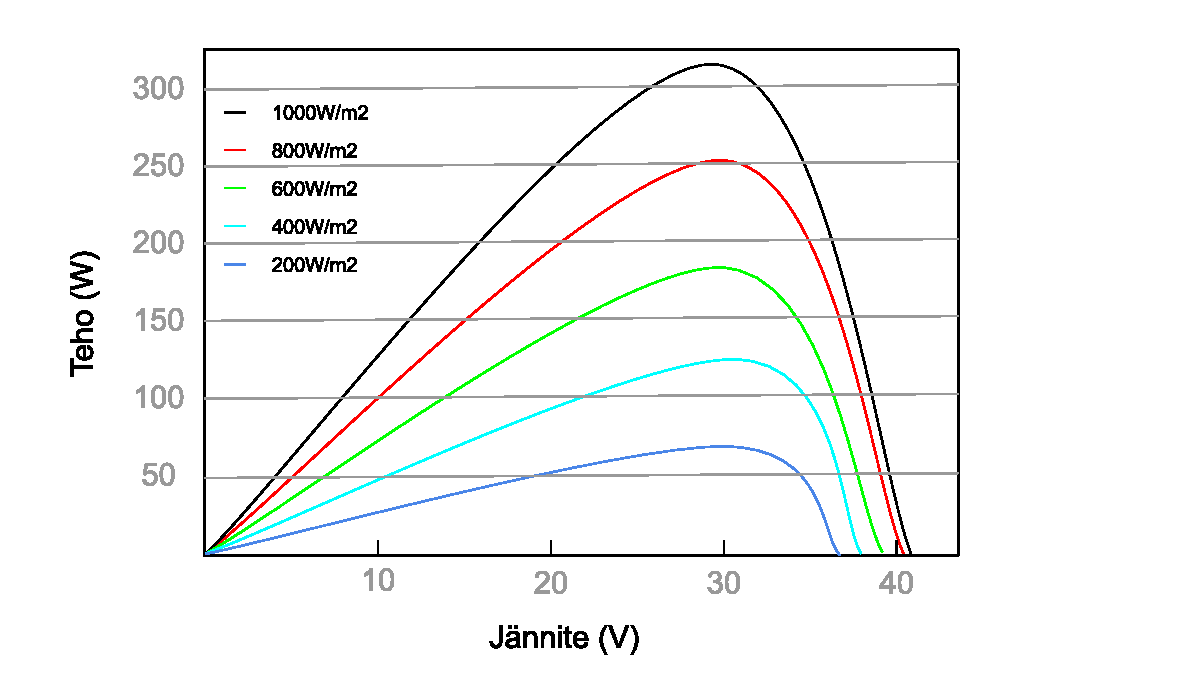
\includegraphics[width=\textwidth]{figures/pvcurve}
    \caption[Esimerkki P--V-käyrästä]{Esimerkki P--V-käyrästä. Perustuen lähteeseen \parencite{JASolar}}
  \end{figure} Kuten kuvasta 2.2 nähdään, P--V-käyrän huippukohdan sijainti vaihtelee valaisutehon mukaan. Tätä käyrän huippukohtaa kutsutaan huipputehopisteeksi (engl. Maximum Power Point, MPP). Se näyttää jännitteen, jolla saavutetaan kennon tai paneelin huipputeho kullakin valaisuteholla.

  Piirillä, jossa on sarjaan kytkettyjä aurinkopaneeleita, on jokaisella paneelilla oma paikallinen huipputehopisteensä, mutta myös koko piirillä on yhteinen globaali huipputehopiste. Globaali huipputehopiste muuttuu varjostusten ja pilvisyyden mukaan koko järjestelmän tasolla ja sitä tarkkailemalla saadaan selville, millä jännitteellä koko järjestelmästä saadaan suurin teho.

\section{Invertterit}
  Invertteri eli vaihtosuuntaaja on laite, joka muuttaa tasasähköä vaihtosähköksi. Invertterin sisääntulojännite vaihtelee käyttötarkoituksen mukaan: kaupalliseen käyttöön tai suurempiin järjestelmiin tarkoitetut laitteet toimivat korkealla, jopa \SI{1500}{\volt} jännitteellä, koska niissä on pidemmät johdotusmatkat ja suurempi määrä paneeleita kytkettynä sarjaan. Kuluttajakäytössä taas voidaan käyttää selvästi pienemmän tason jännitteitä johdotusten ollessa huomattavasti lyhyempiä ja paneeleiden määrän ollessa pienempi.

  Korkeampi jännitetaso keventää huomattavasti tarvittavaa johdotusta, kun virta voidaan pitää pienenä ja siten johtojen läpimitta pienenä. Myös häviöt pienenevät huomattavasti, koska johdoissa syntyvät häviöt kasvavat Ohmin lain
  \begin{equation}
    \textrm{P} = RI^2
  \end{equation}
  mukaan virran suhteen neliöllisenä.

  Invertteri, jolla on valmiudet huipputehopisteen seurantaan (engl. MPP Tracking, MPPT), etsii siihen kytketyn aurinkopaneeliryhmän huipputehopistettä aktiivisesti. Pisteen etsimiseen käytetään monia eri tekniikoita, mutta tämän työn kannalta niiden läpikäynti ei ole relevanttia. Jos käytetty tekniikka on liian herkkä löytämään huipputehopisteitä, se voi valita paikallisen pisteen globaalin sijaan ja aiheuttaa huomattavia tehohäviöitä väärän pisteen valinnalla. \parencite{Joshi&Arora}

  Aurinkopaneeliryhmän tehoa voidaan muuttaa kuormavastusta säätämällä. Huipputehopisteelle löytyy aina sitä vastaava ominaisvastus kaavan
  \begin{equation}
    R_{CH} = \frac{V_{MPP}}{I_{MPP}}
  \end{equation}
  mukaisesti \parencite{Joshi&Arora}, ja invertteri säätää kuormavastuksen ominaisvastuksen mukaiseen arvoon löydettyään järjestelmän huipputehopisteen mukaiset arvot kaavaan.

  Invertterit voidaan jakaa pääosin kolmeen eri tyyppiin järjestelmien topologioiden mukaan: keskusinverttereihin, mikroinverttereihin sekä ketjuinverttereihin. Keskusinvertterit ovat kaupallisissa kohteissa käytettäviä, suuritehoisia inverttereitä, kun taas mikroinvertterit ovat pääosin kuluttajakäyttöön suunnattuja laitteita. Ketjuinvertterit sijoittuvat näiden väliin ja laajan tehoskaalan vuoksi niitä voidaan käyttää molempien tyyppisissä kohteissa.

\subsection{Keskusinvertteri}
  Keskusinvertterin teho on usein hyvin suuri, yli \SI{50}{\kilo\watt}:sta jopa muutamaan megawattiin. Niitä käytetään suurissa aurinkovoimaloissa, joissa ei usein tarvitse miettiä rakennelmien tai puiden aiheuttamia varjostuksia. Tällöin asennuskustannukset pienenevät, sillä suuriin järjestelmiin riittää yksi invertteri.

  Keskusinvertterin huonoja puolia ovat järjestelmän riippuvuus yksittäisestä invertteristä sekä vain muutama huipputehopiste koko järjestelmälle. Tällöin järjestelmässä tulee suuret tehohäviöt, jos esimerkiksi pilvi kulkee osittain paneelikentän yli ja huipputehopiste määräytyy koko järjestelmälle, jolloin täysin auringossa olevien paneelien teho laskee huomattavasti. Käyttökohteiden ja suunnittelun takia tämä ei toisaalta vaikuta merkittävästi järjestelmän tuottoon.

\subsection{Mikroinvertteri}
  Mikroinvertteri on pienitehoinen vaihtosuuntaaja, joka on joko integroitu aurinkopaneelin yhteyteen tai asennettu sen välittömään läheisyyteen. Tämä tarkoittaa, että jokaiselta paneelilta voidaan säätää sen tehoa huipputehopisteen mukaiseksi. Tällöin saadaan epätasaisissa varjostustilanteissa paras mahdollinen teho, kun jokaisesta paneelista voidaan maksimoida teho. Tämä johtuu siitä, että yhden paneelin varjostuminen ei vaikuta muiden paneelien tuottoon, koska paneelit eivät ole kytketty sarjaan.

  Mikroinverttereiltä saadaan hyvin paljon tietoa, koska inverttereiden määrä järjestelmässä on suuri. Tällöin saadaan reaaliaikaisesti kuva järjestelmän toimivuudesta, ja pienetkin virhetilat voidaan korjata niiden ilmentyessä. Toisaalta inverttereiden määrä aiheuttaa haasteita tiedon koostamisessa ja tiedonsiirrossa, koska tieto ei ole välttämättä keskitetysti yhdessä paikassa sellaisenaan, vaan voi vaatia ylimääräisiä komponentteja tiedon keräämiseen.

  Kuluttajapuolen ratkaisuissa tiedonhallinta on usein toteutettu verkkokäyttöliittymällä, jolloin jokainen invertteri on liitetty erilliseen laitteeseen, joka lähettää tiedot valmistajan omaan järjestelmään tiedon koontia varten. Tästä esimerkkinä Enphasen Envoy ja Envertechin EnverBridge, jotka kommunikoivat valmistajan mikroinverttereiden kanssa PLC-väylän kautta. Sen jälkeen laite lähettää tiedot verkkoportaaliin, josta käyttäjä voi seurata paneelien tuotantoa ja järjestelmän toimivuutta. \parencite{Enphase, Envertech}

\subsection{Ketjuinvertteri}
  Ketjuinvertteriin kytketään nimensä mukaisesti sarjaan kytketyistä paneeleista muodostettuja ketjuja. Siinä on usein monta huipputehopisteen seurannan kytkentää, jolloin saadaan seurattua useita huipputehopisteitä invertteriä kohden. Invertterien teho vaihtelee muutamasta kilowatista jopa satoihin kilowatteihin, jolloin sitä voidaan käyttää hyvin erikokoisissa järjestelmissä.

  Teholuokaltaan pienet ketjuinvertterit on suunniteltu käyttäjäystävällisyyshuomioiden, ja esimerkiksi SMA:n ja Huawein invertterit sisältävät integraation valmistajien taustajärjestelmiin. SMA on toteuttanut tämän integraation valmiina laitteelle, kun taas osa Huawein inverttereistä vaatii sovittimen Ethernet-portin, WLAN:in tai matkapuhelinverkon käyttämiseen datasiirrossa.

  SMA:n invertterit käyttävät lisäksi SunSpec Alliancen SunSpec Modbus -standardia, joka toimii Ethernet-verkon välityksellä. Muut standardia hyödyntävät valmistajat voivat kommunikoida suoraan SMAn inverttereiden kanssa standardoinnin takia. Huawei käyttää myös Modbus-protokollaa, mutta se ei ole SunSpec Alliancen standardoima. Tämä tarkoittaa, että Huawein kanssa kommunikoitaessa sille on räätälöitävä ohjelmistoa datan lukemiseksi. \parencite{SMAManual, Huawei}

  Modbusin hyödyntäminen mahdollistaa muiden valmistajien tuotteiden kommunikaation inverttereiden kanssa. Yhteinen standardi helpottaa suurissa järjestelmissä eri valmistajien tuotteiden yhteensopivuuden kanssa, mutta ylipäätään Modbusin käyttö antaa mahdollisuuden kolmannen osapuolen tuotteiden liittämiseen.

\section{Järjestelmien tuotto-ominaisuudet}
  Aurinkosähköjärjestelmät ovat sähköntuottajina teholtaan nopeasti muuttuvia. Niiden tuoton ennustaminen on jokseenkin mahdollista päivätasolla, mutta tuntitehon ennustaminen sääennusteen perusteella on jo haastavaa. Toisaalta, kun tuotannon määrä verkossa kasvaa, eri sijainnissa olevat järjestelmät tasaavat näitä tuotannon vaihteluita ja suuressa kuvassa niiden kokonaistuotantokäyrä ''pehmenee''. Tätä on tutkittu tuulivoiman osalta, joka sähköntuottajana on aurinkosähkön kanssa samankaltainen. \parencite{FluctuationIssues}
  
  Nykyisellä keskitettyyn sähköntuotantoon rakennetulla verkolla aurinkosähköjärjestelmät tuovat haasteita, sillä pientuotantoa lisätessä johtolähtöjen jännitetasot nousevat ja verkon suojaustoimintoja voidaan joutua päivittämään. Esimerkiksi mikrotuotanto voi aiheuttaa vikavirtasuojauksen virhelaukaisun, mikäli tuotanto on lähellä muuntajan kiskoa ja se alkaa syöttämään läheisen lähdön vikatilanteessa vikavirtaa kiskoa kohti. Tällöin terveessä lähdössä tapahtuu virhelaukaisu. \parencite{Mikrotuotanto}
  
  Aurinkosähkön osuuden kasvaminen sähköntuotannossa lisää säädettävän tuotantokapasiteetin tarvetta sähkömarkkinoilla. Päivän aikana nettotehonmuutos on suuri, kun aurinkosähköjärjestelmät alkavat tuottaa sähköä samalla, kun kysyntä laskee ihmisten lähtiessä töihin. Vastaavasti sama tapahtuu illalla kun ihmiset palaavat töistä ja järjestelmän tuottoteho laskee. Tätä ilmiötä kuvaa niin sanottu ''duck''-käyrä, joka nähdään kuvassa 2.3. \begin{figure}
    \centering
    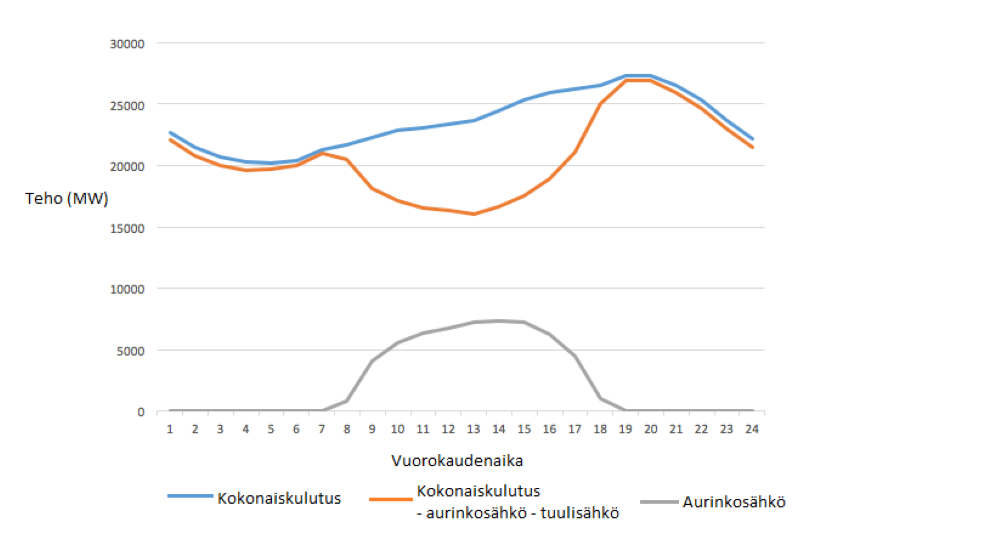
\includegraphics[width=1.1\textwidth]{figures/Duck_curve.png}
    \caption{''Duck''-käyrä}
  \end{figure} Se kuvaa säädettävän energiatuotannon keskimääräistä hetkellistä tuotantotehoa vuorokauden aikana. \parencite{duckCurve}

  Tuotantokapasiteetin tarvetta voidaan helpottaa energiavarastojen avulla, jolloin päivän energiantuotantoa saadaan siirrettyä illan huippukuormituksen ajalle. Energiavarastot tasaavat myös aurinkosähkön tuotannon ailahtelevuutta. Ongelmana energiavarastojen määrän lisääntymisessä on kuitenkin niiden korkea hankintahinta ja niistä saatavat hyödyt.

  Yksittäiselle kuluttajalle energiavarastoista saatavat hyödyt tulevat tuotetun sähkön hyödyntämisestä kalliimman sähkönhinnan aikaan, sillä kuluttajan saama tuotto myydystä sähköstä on pienempi kuin itse kulutetun energian hinta. Lisäksi tuottaja voi haluta kodistaan enemmän energiaomavaraisen ja käyttää tuotetun sähkön kokonaan itse. Mikäli kuluttajalla ei ole kulutusjoustoon soveltuvia laitteita, voi se hyödyntää energiavarastoa tuotetun sähkön hyödyntämiseen tuotantoajan ulkopuolella.
  
  Tuottajalla on taas useampi syy energiavarastojen hyödyntämiseen. Matala sähköstä saatava markkinahinta on myös tuottajalla syy hyödyntää energiavarastoa, varsinkin jos hinta on tuotantohuipun aikaan matala. Verkkokoodi määrittelee tuotantolaitoksien sähköverkkoon liittämisvaatimukset. Tulevaisuudessa se voi pakottaa tuotantolaitokset investoimaan energiavarastoon sähköverkon vakauden ja jännitteen laadun ylläpitämiseksi. Vaikka verkkokoodi ei pakottaisi investoimaan energiavarastoon, voi se olla kannattavaa, jos verkonhaltija joutuisi vahvistamaan verkkoa ja liittyjän kustannukset nousisivat muuten. Tariffihinnoittelun muuttuminen tulevaisuudessa tehopohjaiseksi kannustaa yrityksiä investoimaan myös energiavarastoihin, sillä niillä voidaan loiventaa kulutushuippua, jolloin tariffimaksu pienenee.
